\documentclass[10pt,onecolumn]{article}
\usepackage[margin=0.8in]{geometry}
\usepackage[utf8]{inputenc}
\usepackage[T1]{fontenc}
\usepackage{mathptmx}
\usepackage{amsmath,amssymb,bm}
\usepackage{graphicx,booktabs,tabularx,array,multirow}
\usepackage{microtype,cite}
\usepackage{caption}
\captionsetup{font=small,labelfont=bf,labelsep=period}
\usepackage{xcolor}
\definecolor{ink}{HTML}{172C43}
\definecolor{accent}{HTML}{007C83}
\usepackage{hyperref}
\hypersetup{colorlinks=true,urlcolor=accent,citecolor=ink,linkcolor=ink,pdftitle={Temporal Retiming Attacks on Hybrid Quantum Spiking Classifiers}}
\usepackage{url}
\urlstyle{same}
\Urlmuskip=0mu plus 2mu\relax
\makeatletter
\g@addto@macro\UrlBreaks{\do\-\do\_\do\?\do\&\do\=}
\makeatother
% Keep one bibliography entry together across columns/pages.
\let\originalthebibliography\thebibliography
\renewcommand{\thebibliography}[1]{\originalthebibliography{#1}\interlinepenalty=10000\relax}
\newcolumntype{L}{>{\raggedright\arraybackslash}X}
\newcolumntype{C}{>{\centering\arraybackslash}X}
\newcolumntype{R}{>{\raggedleft\arraybackslash}X}
\setlength{\emergencystretch}{1.5em}
\raggedbottom
\setlength{\columnsep}{0.25in}
\setlength{\textfloatsep}{11pt plus 2pt minus 2pt}
\setlength{\dbltextfloatsep}{12pt plus 2pt minus 2pt}
\setlength{\floatsep}{9pt plus 2pt minus 2pt}
\renewcommand{\topfraction}{0.95}
\renewcommand{\dbltopfraction}{0.95}
\renewcommand{\textfraction}{0.05}
\renewcommand{\floatpagefraction}{0.85}
\setcounter{topnumber}{3}
\setcounter{dbltopnumber}{2}

\hypersetup{pdftitle={Supplementary Material: Temporal Retiming Attacks}}
\renewcommand{\thesection}{S\arabic{section}}
\renewcommand{\thesubsection}{\thesection.\arabic{subsection}}
\renewcommand{\thetable}{S\arabic{table}}
\renewcommand{\thefigure}{S\arabic{figure}}
\renewcommand{\theequation}{S\arabic{equation}}
\setlength{\parindent}{1em}
\setlength{\parskip}{2pt}
\newcommand{\tabnote}[1]{\par\vspace{3pt}{\small\raggedright\noindent #1\par}}
\newcommand{\rref}[1]{\textup{[R#1]}}
\title{\vspace{-1.5em}Supplementary Material\\[4pt]
\large Temporal Retiming Attacks on Hybrid Quantum Spiking Classifiers}
\author{Authors withheld for review}
\date{}
\begin{document}
\maketitle
\vspace{-1.2em}
\noindent This supplement preserves completed supporting experiments and the full paired timestamp comparison. Historical studies are not additional final-model N-MNIST robustness evaluations. Every section states the model, partition and evidence boundary needed for interpretation. Numerical values are transcribed from preserved reports; model training, attacks and original independent audits were not rerun during preparation. Source identifiers \rref{1}--\rref{10} are mapped to exact repository paths in Section~\ref{sec:evidence}.

\section{Development of the hybrid architecture}
\label{sec:development}
The selected development configurations are summarized in Table~\ref{tab:development} and Figure~\ref{fig:development}. The earlier eight-dimensional frontend differs from the final 32-dimensional \texttt{wide4} frontend. Different training stages, continuation histories and budgets prevent causal attribution of the validation changes to a single circuit component. These are validation-only model-development results, rather than a controlled ablation establishing quantum advantage \rref{1}.

\begin{table}[!htbp]
\centering
\caption{Selected quantum-head and frontend development results.}
\label{tab:development}
\small
\begin{tabularx}{\linewidth}{L C R L}
\toprule
Configuration & Validation accuracy (\%) & Parameters & Scope \\
\midrule
Quantum v1 & 86.16 & 7,026 & Earlier 8D frontend \\
Selected quantum head v2 & 92.60 & 7,130 & Earlier 8D frontend \\
\texttt{wide4} classical control & 97.80 & 38,122 & 32D frontend; seed 42 \\
Final QSNN-v3 & 97.06 & 40,762 & 32D frontend; seed 42 \\
\bottomrule
\end{tabularx}
\tabnote{Sources: \rref{1} and companion frontend/quantum-head development reports. Configuration changes and unequal training stages preclude a component-wise causal interpretation.}
\end{table}

\begin{figure}[!htbp]
\centering
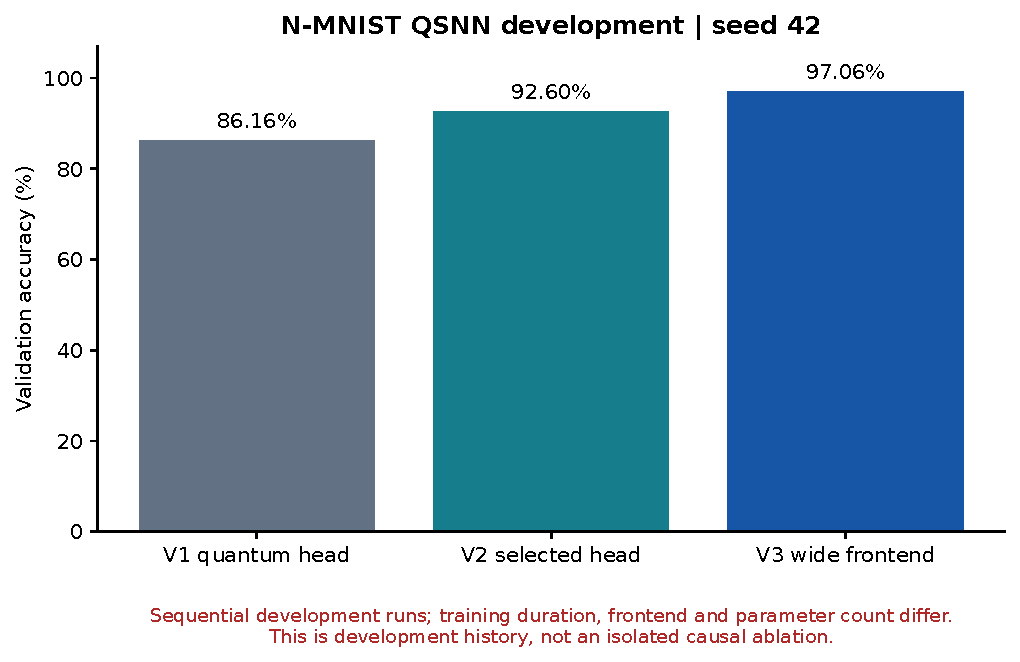
\includegraphics[width=0.93\linewidth]{figures/fig10_qsnn_development.pdf}
\caption{Validation-only development trajectory. Runs differ in frontend dimensions and training stages. The plot documents model development and is not a controlled ablation of quantum advantage \rref{1}.}
\label{fig:development}
\end{figure}

\subsection{Frozen final-model training details}
All five QSNN-v3 runs share one hash-verified seed-42 pretrained frontend and one stratified 55,000/5,000 training/validation partition. The frontend is frozen for the first two epochs and then optimized while its BatchNorm layers remain in evaluation mode. Architecture and hyperparameters are frozen across seeds 42, 123, 777, 2026 and 6543. The official test partition is not instantiated for the final hybrid campaign \rref{1}.

AdamW uses weight decay $10^{-4}$, with learning rates $5\times10^{-5}$ for the extractor, $2.5\times10^{-4}$ for latent projection and circuit, and $10^{-3}$ for the classifier. Training uses batch size 256, a maximum of 40 epochs and gradient clipping at norm 1. The ReduceLROnPlateau schedule uses factor 0.5, patience 2 and minimum learning rate $10^{-5}$. Checkpoint selection prioritizes validation accuracy and then validation loss; early stopping has patience 6 after at least eight epochs. The frontend uses float16 autocast, while circuit inputs are float32 and state amplitudes are complex64. These choices describe the simulated implementation and imply no quantum speedup.

The selected epochs are 37, 24, 40, 38 and 40; recorded runtimes are 1,200.00, 938.80, 1,245.30, 1,251.55 and 1,237.35~s, respectively. The seed-42 process was externally terminated during epoch 38, after saving its epoch-37 best checkpoint; that checkpoint was reloaded and evaluated for the reported result. Between-seed variability is conditional on shared pretraining and split, rather than variability across independently pretrained pipelines.

\clearpage
\section{Earlier binary-grid budget sweep}
\label{sec:historicalgrid}
The historical representation-matched binary custom SNN has 98.73\% clean accuracy on the complete 10,000-example official test partition. Its nine-budget attack sweep uses 1,000 clean-correct examples and a different checkpoint, temporal binning and manifest from the controlled four-model study. In particular, its $B_\infty=1$ ASR is 82.9\%, whereas the controlled campaign's custom-model rate is 100.0\%. Both values are retained as results of separate experiments \rref{5}.

\begin{table}[!htbp]
\centering
\caption{Historical binary-grid attack sweep.}
\label{tab:historicalgrid}
\small
\begin{tabularx}{\linewidth}{L C C C C C}
\toprule
Budget & Successes / $N$ & ASR (\%) & Actual $B_\infty$ & Actual $B_1$ & Actual $B_0$ \\
\midrule
$B_\infty=1$ & 829 / 1,000 & 82.9 & 1--1 & 568--2,604 & 568--2,604 \\
$B_\infty=2$ & 1,000 / 1,000 & 100.0 & 2--2 & 840--4,231 & 573--2,766 \\
$B_\infty=3$ & 1,000 / 1,000 & 100.0 & 3--3 & 1,092--5,545 & 576--2,841 \\
$B_1=500$ & 1,000 / 1,000 & 100.0 & 3--9 & 500--500 & 268--463 \\
$B_1=750$ & 1,000 / 1,000 & 100.0 & 4--9 & 750--750 & 364--615 \\
$B_1=1{,}000$ & 1,000 / 1,000 & 100.0 & 6--9 & 1,000--1,000 & 438--790 \\
$B_0=200$ & 1,000 / 1,000 & 100.0 & 8--9 & 683--955 & 200--200 \\
$B_0=300$ & 1,000 / 1,000 & 100.0 & 8--9 & 1,051--1,403 & 300--300 \\
$B_0=400$ & 1,000 / 1,000 & 100.0 & 9--9 & 1,369--1,913 & 400--400 \\
\bottomrule
\end{tabularx}
\tabnote{All realized budget ranges are transcribed from the historical report \rref{5}; they are not regenerated from attack tensors. Budget families have different units: maximum displacement, total displacement and number of retimed packets.}
\end{table}

\begin{figure}[!htbp]
\centering
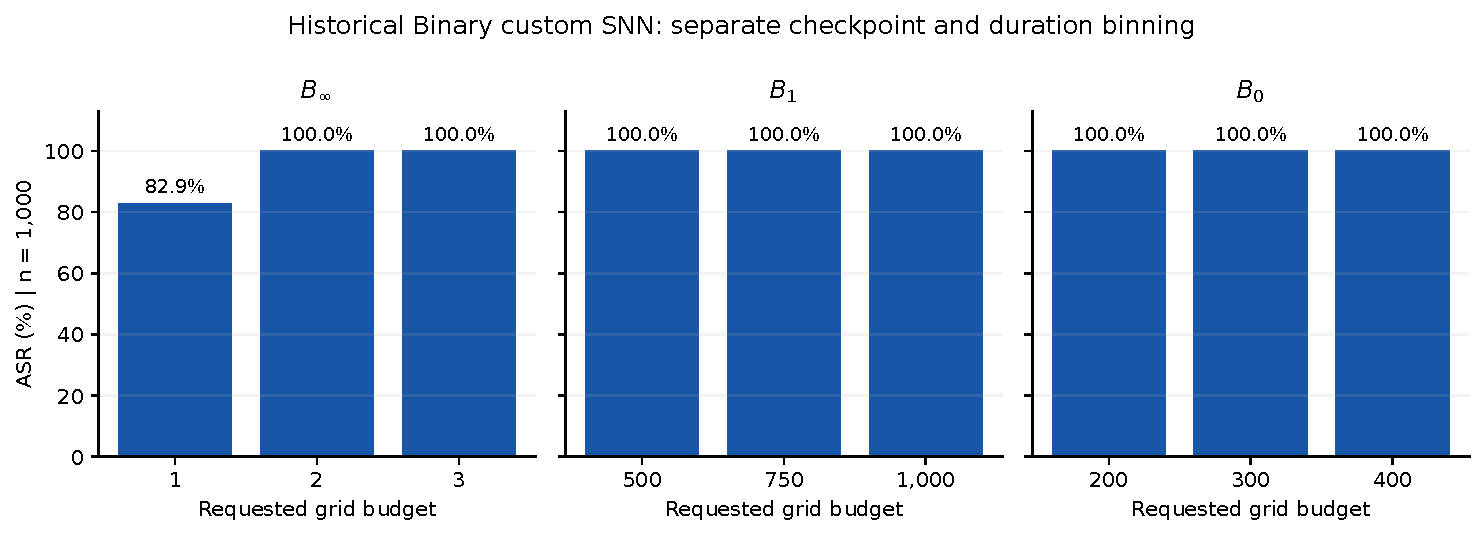
\includegraphics[width=0.95\linewidth]{figures/fig05_historical_binary_budgets.pdf}
\caption{Historical binary-grid success rates for three budget families. Units differ by family. This sweep is not merged with the controlled four-model results \rref{5}.}
\label{fig:historicalgrid}
\end{figure}

\begin{figure}[!htbp]
\centering
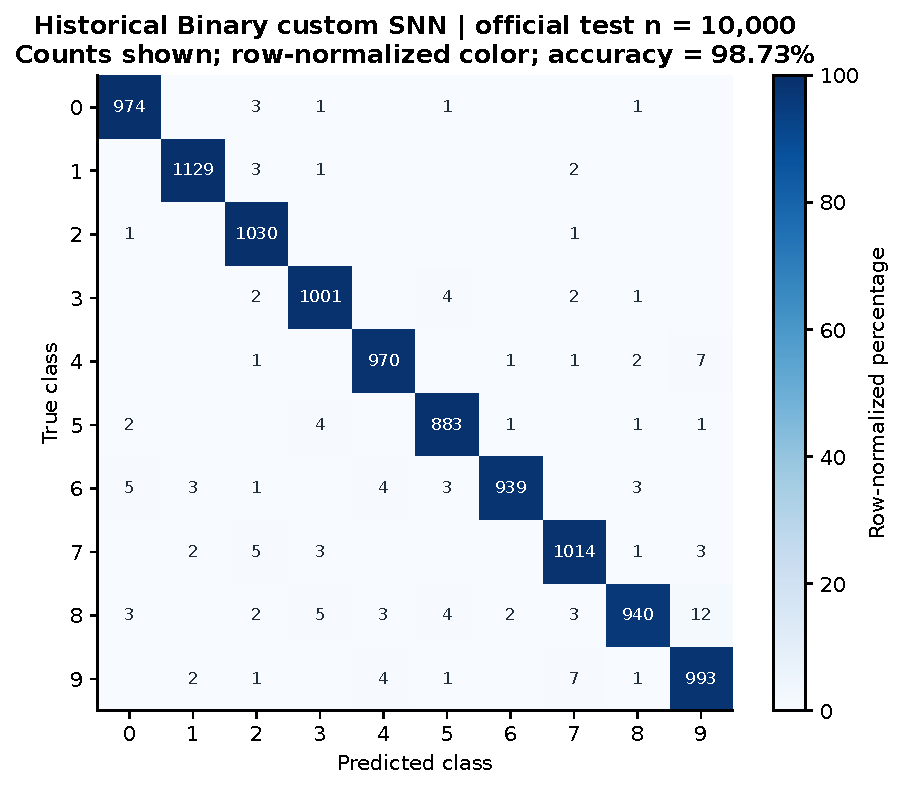
\includegraphics[width=0.69\linewidth]{figures/fig06_binary_confusion.pdf}
\caption{Clean confusion matrix of the historical binary custom SNN on 10,000 official-test examples. The diagonal sums to 9,873, giving 98.73\% accuracy. This is not a QSNN-v3 confusion matrix \rref{5}.}
\label{fig:confusion}
\end{figure}

The corrected integer-grid campaign separately freezes clean-correct manifests using only strict integer-grid predictions. Its status report lists 8 of 33 attack conditions complete and 25 remaining, with the next condition seed 42 and $B_0=300$. The preserved final ASR summary is absent. Historical integer attack values are excluded from the corrected campaign summary because they cannot replace its required corrected artifacts \rref{5}.

\clearpage
\section{Clean neuromorphic baselines}
\label{sec:neuromorphic}
\begin{table}[!htbp]
\centering
\caption{Three-seed clean classical baseline accuracy.}
\label{tab:neuromorphic}
\small
\begin{tabularx}{\linewidth}{L L C L}
\toprule
Dataset & Representation & Mean $\pm$ SD (\%) & Evaluation scope \\
\midrule
N-MNIST & Binary grid & $98.5167\pm0.2203$ & Official test \\
N-MNIST & Integer grid & $98.3867\pm0.2146$ & Official test \\
DVS-Gesture & Binary grid & $81.3131\pm2.8930$ & Official test \\
DVS-Gesture & Legacy integer & $83.0808\pm4.6289$ & Normalized counts \\
CIFAR10-DVS & Binary grid & $50.4000\pm2.0075$ & Frozen 10\% test split \\
CIFAR10-DVS & Legacy integer & $46.2000\pm6.1733$ & Normalized counts \\
\bottomrule
\end{tabularx}
\tabnote{Seeds 42, 123 and 777. DVS-Gesture and CIFAR10-DVS rows historically labeled ``integer'' retain legacy normalized-count preprocessing and are \textbf{non-comparable} with strict integer grids \rref{6}.}
\end{table}

\begin{figure}[!htbp]
\centering
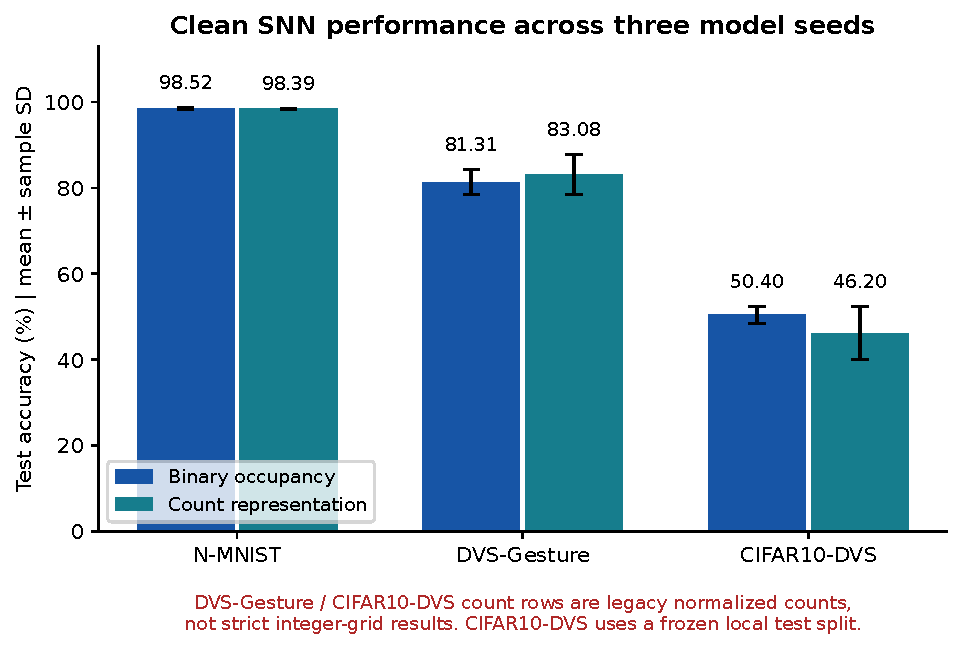
\includegraphics[width=0.95\linewidth]{figures/fig07_neuromorphic_clean.pdf}
\caption{Classical clean accuracy across three seeds. Binary and N-MNIST integer rows are representation-matched. DVS-Gesture and CIFAR10-DVS integer rows retain legacy normalization and do not establish strict-integer performance \rref{6}.}
\label{fig:neuromorphic}
\end{figure}

N-MNIST uses all 10,000 official-test examples and DVS-Gesture all 264 official-test examples per seed. CIFAR10-DVS uses a frozen class-stratified 10\% split of 1,000 examples because there is no official train/test partition in this protocol. These are clean SNN baselines; they provide no additional QSNN attack or defense results.

\clearpage
\section{Iris attacks and quantum-state diagnostics}
\label{sec:iris}
\begin{table}[!htbp]
\centering
\caption{Historical Iris attack means across five model seeds.}
\label{tab:iris}
\fontsize{9}{11}\selectfont
\begin{tabularx}{\linewidth}{@{}c C C C C@{}}
\toprule
$100\epsilon/T$ & Classical ASR (\%) & Adaptive TEMP ASR (\%) & Classical $1-F$ & Adaptive TEMP $1-F$ \\
\midrule
2 & $8.64\pm6.22$ & $8.64\pm6.22$ & $0.000987\pm0.000000$ & $0.000980\pm0.000006$ \\
5 & $19.18\pm8.28$ & $19.18\pm8.28$ & $0.006109\pm0.000039$ & $0.005766\pm0.000103$ \\
10 & $32.85\pm9.67$ & $33.54\pm10.23$ & $0.024069\pm0.000276$ & $0.021953\pm0.000473$ \\
\bottomrule
\end{tabularx}
\tabnote{Seed-specific clean-correct denominators are 29, 29, 29, 23 and 27. ASR means average seed-specific ratios rather than pooling them. Drift values are reported pure product-state diagnostics \rref{8}.}
\end{table}

\begin{figure}[!htbp]
\centering
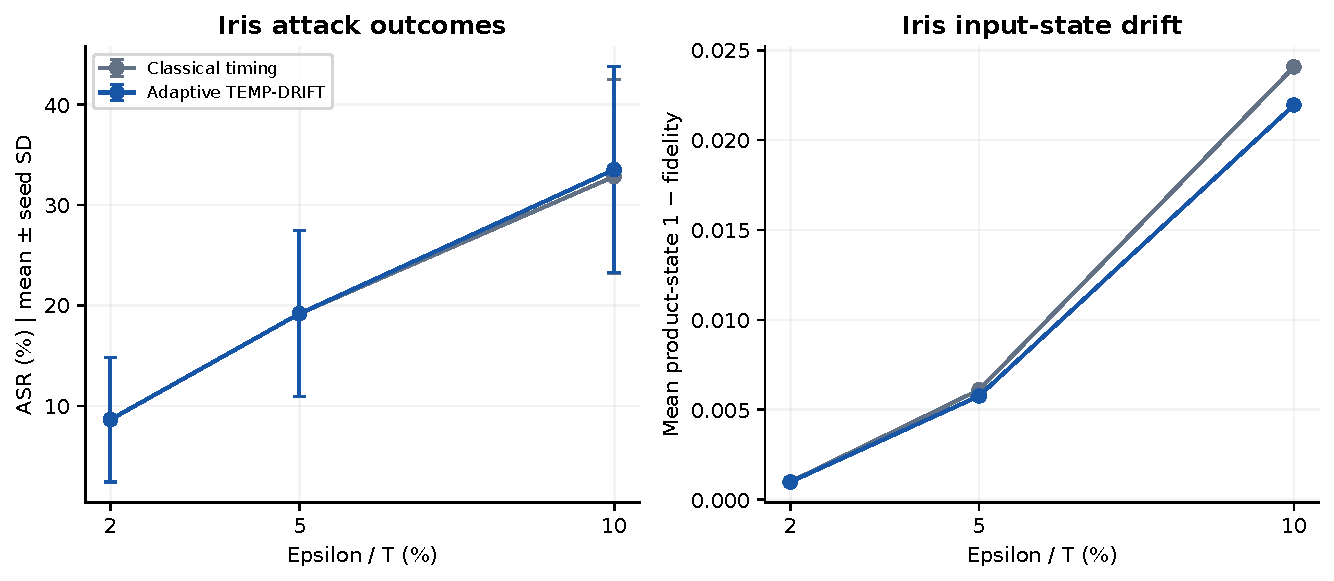
\includegraphics[width=0.95\linewidth]{figures/fig08_iris_attack_and_drift.pdf}
\caption{Earlier Iris ASR and state-drift diagnostics. At 10\%, TEMP has one extra attack success, but the classical timing attack has larger mean drift. Error bars show between-model-seed variability on small evaluation subsets \rref{8}.}
\label{fig:iris}
\end{figure}

At 10\%, classical successes total 46/137 and adaptive TEMP successes 47/137 across the seed-specific populations. These pooled observations repeat the underlying dataset across model seeds, so they are not 137 independent subjects. The exact paired count table has zero classical-only and one TEMP-only success; it does not support attack superiority. The drift quantity refers to the Iris encoding and must not be substituted for an unmeasured N-MNIST circuit-state distance.

\section{Earlier Iris regularization and mechanism gate}
\label{sec:regularization}
\begin{table}[!htbp]
\centering
\caption{Earlier Iris regularization replication.}
\label{tab:regularization}
\small
\begin{tabularx}{\linewidth}{L C C L}
\toprule
Measure & Baseline & Regularized model & Interpretation \\
\midrule
Clean accuracy (\%) & $84.00\pm9.25$ & $84.00\pm8.63$ & Mean change 0; one seed improves and one degrades \\
PGD 10\% paired ASR (\%) & $25.58\pm10.07$ & $24.09\pm8.45$ & Two rescued and zero broken across 125 repeated observations \\
Reference TEMP 10\% & --- & One rescued observation & Improvement confined to seed 42 \\
Gradient TEMP & --- & One rescued observation per $\tau$ & No improvement in the other four seeds \\
\bottomrule
\end{tabularx}
\tabnote{Fixed split seed 42; five paired model seeds; $\lambda_q=5$ and $\lambda_{\rm pred}=0$. This is representation regularization, not tomography detection. Source: \path{results/phase153_results.md}, under \rref{9}.}
\end{table}

The Phase-21 confirmatory mechanism gate subsequently fails two of four criteria. Its split-level confidence interval crosses zero, so Stage B is blocked and no candidate defense is trained. An audit PASS in that report means that the negative gate result was handled according to the protocol; it does not mean that the proposed defense succeeded. No hidden-test defense result is inferred from nonexecution \rref{9}.

\section{MNIST development and SHD classical testing}
\label{sec:mnistshd}
\begin{table}[!htbp]
\centering
\caption{Seed-42 MNIST clean validation screen.}
\label{tab:mnist}
\small
\begin{tabularx}{\linewidth}{C C C C}
\toprule
PCA dimensions & Explained variance (\%) & Validation accuracy (\%) & Macro-F1 (\%) \\
\midrule
16 & 87.64 & 86.80 & 86.75 \\
24 & 95.42 & 85.30 & 85.24 \\
32 & 98.42 & 83.55 & 83.46 \\
\bottomrule
\end{tabularx}
\tabnote{Downsampled $8\times8$ MNIST and a separate classifier; one development seed. Runs have different continuation and timeout histories. No attack or defense conclusion follows \rref{7}.}
\end{table}

\begin{figure}[!htbp]
\centering
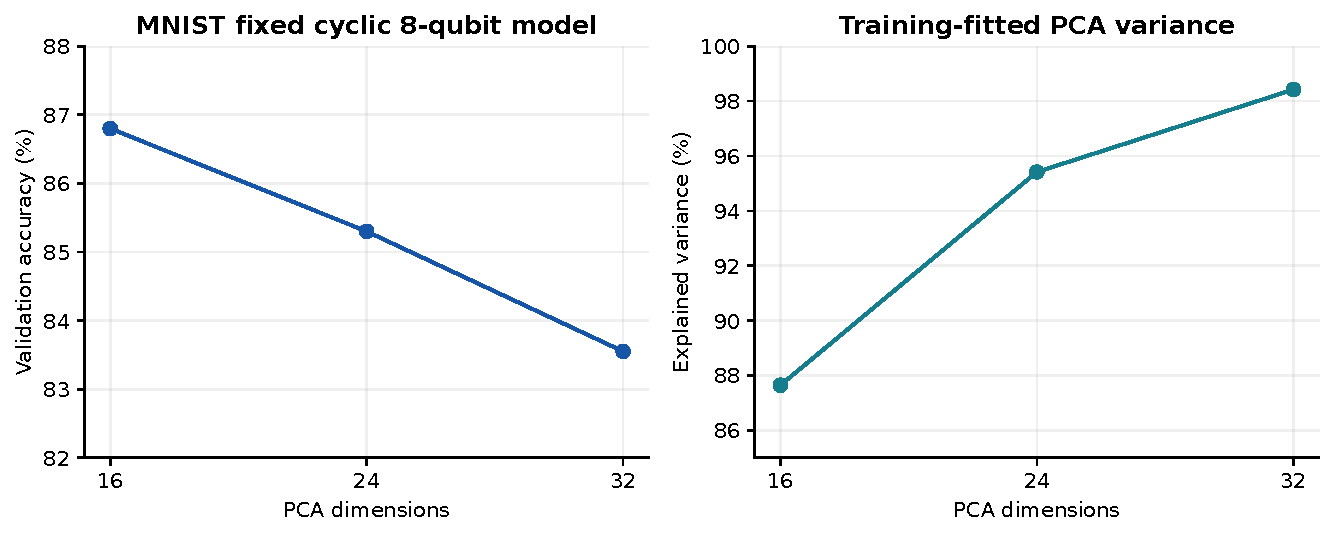
\includegraphics[width=0.86\linewidth]{figures/fig09_mnist_pca_ablation.pdf}
\caption{MNIST validation accuracy versus PCA dimension. Retaining more variance did not improve validation accuracy in these development runs. This is not a matched-training-budget ablation \rref{7}.}
\label{fig:mnist}
\end{figure}

\begin{table}[!htbp]
\centering
\caption{SHD classical SNN official-test re-audit.}
\label{tab:shd}
\small
\begin{tabularx}{0.78\linewidth}{C C C}
\toprule
Seed & Test accuracy (\%) & Macro-F1 (\%) \\
\midrule
42 & 65.7686 & 64.6785 \\
123 & 69.7880 & 69.1100 \\
777 & 66.2102 & 65.6300 \\
2026 & 64.0018 & 63.1983 \\
6543 & 64.1784 & 63.9006 \\
Mean $\pm$ SD & $65.9894\pm2.3322$ & $65.3035\pm2.3123$ \\
\bottomrule
\end{tabularx}
\tabnote{The historical re-audit reports that recomputed values match its previous test values. This is classical SNN testing on a previously accessed test set, not a QSNN robustness study. Source: \path{results/shd_snn_test_reaudit_report.md}, under \rref{10}.}
\end{table}

\clearpage
\section{Quantum-state notation and monitoring bounds}
\label{sec:quantum}
\subsection{State angles, Bloch vector and density-matrix sign}
For an individually encoded one-qubit state, the state-amplitude angle $\theta(t)$ and phase $\phi(t)$ define
\begin{equation}
\lvert\psi(t)\rangle=\cos\theta(t)\lvert0\rangle+
 e^{i\phi(t)}\sin\theta(t)\lvert1\rangle.
\label{eq:state}
\end{equation}
With the usual Pauli matrices, its Bloch vector is
\begin{equation}
\mathbf r=\bigl(\sin2\theta\cos\phi,\ \sin2\theta\sin\phi,\ \cos2\theta\bigr).
\label{eq:bloch}
\end{equation}
The density matrix and its upper-right entry are therefore
\begin{equation}
\rho=\frac12\bigl(I+\mathbf r\cdot\boldsymbol\sigma\bigr),
\qquad \rho_{01}=\frac{r_x-i r_y}{2}.
\label{eq:density}
\end{equation}
This fixes the conjugation/sign ambiguity in the original appendix.

The repository's Iris angle encoder returns $\theta=\pi t/(2T)$, while a conventional $R_Y$ gate uses rotation angle $2\theta$. Its amplitude option uses $\theta=\arccos\sqrt{1-t/T}$; its phase option uses $\theta=\pi/4$ and $\phi=2\pi t/T$. State-amplitude angles and rotation-gate angles must therefore be distinguished. The N-MNIST latent circuit has a separate learned angle map and is not an ensemble average of independent per-event qubits.

\subsection{Squared fidelity and the pure-versus-ensemble distinction}
We use squared Uhlmann fidelity,
\begin{equation}
F(\rho,\sigma)=\left[\operatorname{Tr}\sqrt{\sqrt\rho\,\sigma\sqrt\rho}\right]^2.
\label{eq:fidelity}
\end{equation}
For pure product states $\lvert\Psi\rangle=\bigotimes_q\lvert\psi_q\rangle$ and $\lvert\Phi\rangle=\bigotimes_q\lvert\phi_q\rangle$, the implemented squared overlap and trace distance are
\begin{equation}
F=\lvert\langle\Psi\vert\Phi\rangle\rvert^2
 =\prod_q\lvert\langle\psi_q\vert\phi_q\rangle\rvert^2,
\qquad D_{\rm tr}=\sqrt{1-F}.
\label{eq:product}
\end{equation}
A mixed event ensemble instead has the form
\begin{equation}
\rho_{\rm ens}=\frac1N\sum_{i=1}^{N}
\lvert\psi(t_i)\rangle\langle\psi(t_i)\rvert
\label{eq:ensemble}
\end{equation}
and requires the mixed-state fidelity in Eq.~\eqref{eq:fidelity}. The pure product overlap and mixed ensemble fidelity are not interchangeable computational objects.

A one-qubit state is completely determined by its Bloch vector. Identical Bloch vectors imply identical density matrices and zero quantum Jensen--Shannon divergence; there is no additional phase difference hidden from all three Pauli expectations for a single-qubit density matrix. For eight qubits, identical local marginals do not imply identical joint states. A proposed local monitor must recognize this distinction.

\subsection{A simultaneous finite-shot error bound}
For $N_{\rm basis}$ independently estimated observables with outcomes $\pm1$ and $n$ shots per observable, Hoeffding's inequality and a union bound give
\begin{equation}
\Pr\!\left[\max_j\lvert\widehat r_j-r_j\rvert>\delta\right]
\leq 2N_{\rm basis}\exp\!\left(-\frac{n\delta^2}{2}\right).
\label{eq:hoeffdingtail}
\end{equation}
Thus a simultaneous absolute error at most $\delta$ with failure probability at most $\eta$ is ensured by
\begin{equation}
n\geq\frac{2}{\delta^2}\ln\!\frac{2N_{\rm basis}}{\eta}.
\label{eq:shots}
\end{equation}
For three one-qubit Pauli bases and a balanced total budget $M=3n$,
\begin{equation}
\delta=\sqrt{\frac{6}{M}\ln\!\frac{6}{\eta}}.
\label{eq:balancedshots}
\end{equation}
At $\eta=0.05$, this continuous balanced-budget expression gives $\delta\approx0.536$ for $M=100$ and $\delta\approx0.059$ for $M=8{,}192$. Integer shot allocations use $n=\lfloor M/3\rfloor$ per basis and slightly increase the bound. These are theoretical conservative simultaneous bounds, not measured detector sensitivity, and do not give full-register tomography complexity.

No final N-MNIST tomography threshold, ROC/AUC, false-positive rate, finite-shot sensitivity, detection latency or adaptive-attack result is available. Monitoring remains a proposal, and the Iris regularization results in Section~\ref{sec:regularization} are a different intervention.

\section{Complete paired timestamp comparison and supporting diagnostics}
\label{sec:paired}
\subsection{Population, duration convention and computation}
All conditions use the same 100 seed-42 validation examples, with ten per class, correctly classified by both frozen models before attack. They are not independent repeat samples across conditions. The timestamp protocol preserves event coordinates, polarity, count, labels and identities while enforcing nondecreasing times and the clean recording endpoints. In timestamp units the implemented duration and displacement constraint are
\begin{equation}
D=t_N-t_1+1,\qquad \epsilon=\epsilon_fD,\qquad
\lvert t_i'-t_i\rvert\leq\epsilon,
\quad t_1\leq t_i'\leq t_N,\quad t_i'\leq t_{i+1}'.
\label{eq:timestamp}
\end{equation}
The added unit matches the code's inclusive duration convention; it should not be dropped when reproducing budgets. The ten-bin adapter uses the clean recording endpoints and this duration, with hard accumulation in the forward pass and a surrogate backward interpolation \rref{2}.

PGD uses 21 candidate evaluations, 41 attack-internal forwards and 20 backwards. TEMP uses $Q$ candidate/forward evaluations and zero backwards. Candidate matching sets $Q=21$; forward matching sets $Q=41$. Elapsed-time calibration chooses $Q=4{,}000$ for QSNN-v3 and $Q=1{,}600$ for SNN, yielding median TEMP/PGD runtime ratios 0.978 and 1.083. Two verification forwards per new record are excluded from attack timing. No backward-to-forward conversion factor is assumed \rref{3}.

\begin{table}[!htbp]
\centering
\caption{Complete paired timestamp outcomes. Every row has $N=100$ joint clean-correct validation examples. Success counts are also ASR percentages.}
\label{tab:paired}
\fontsize{9}{11}\selectfont
\setlength{\tabcolsep}{4pt}
\begin{tabularx}{\linewidth}{@{}L l r r r r r r r r@{}}
\toprule
Condition & Victim & $100\epsilon_f$ & PGD & TEMP & $b$ & $c$ & Both & Neither & Exact $p$ \\
\midrule
Original fixed budget & SNN & 5 & 0 & 0 & 0 & 0 & 0 & 100 & 1 \\
Original fixed budget & SNN & 10 & 0 & 1 & 0 & 1 & 0 & 99 & 1 \\
Original fixed budget & QSNN-v3 & 5 & 3 & 4 & 0 & 1 & 3 & 96 & 1 \\
Original fixed budget & QSNN-v3 & 10 & 3 & 5 & 0 & 2 & 3 & 95 & 0.5 \\
21 candidates & SNN & 5 & 0 & 0 & 0 & 0 & 0 & 100 & 1 \\
21 candidates & SNN & 10 & 0 & 0 & 0 & 0 & 0 & 100 & 1 \\
21 candidates & QSNN-v3 & 5 & 3 & 4 & 0 & 1 & 3 & 96 & 1 \\
21 candidates & QSNN-v3 & 10 & 3 & 3 & 0 & 0 & 3 & 97 & 1 \\
41 forwards & SNN & 5 & 0 & 0 & 0 & 0 & 0 & 100 & 1 \\
41 forwards & SNN & 10 & 0 & 0 & 0 & 0 & 0 & 100 & 1 \\
41 forwards & QSNN-v3 & 5 & 3 & 4 & 0 & 1 & 3 & 96 & 1 \\
41 forwards & QSNN-v3 & 10 & 3 & 3 & 0 & 0 & 3 & 97 & 1 \\
Elapsed time & SNN & 5 & 0 & 0 & 0 & 0 & 0 & 100 & 1 \\
Elapsed time & SNN & 10 & 0 & 1 & 0 & 1 & 0 & 99 & 1 \\
Elapsed time & QSNN-v3 & 5 & 3 & 4 & 0 & 1 & 3 & 96 & 1 \\
Elapsed time & QSNN-v3 & 10 & 3 & 5 & 0 & 2 & 3 & 95 & 0.5 \\
\bottomrule
\end{tabularx}
\tabnote{$b$: PGD-only success; $c$: TEMP-only success. The original fixed-budget condition is distinct from candidate, forward and elapsed-time matching. Identical aggregate counts do not imply additional independent observations. Exact two-sided paired $p$-values are checked from the preserved discordant counts \rref{3}.}
\end{table}

At 5\% on QSNN-v3, the three joint successes and one TEMP-only success give exact paired $p=1$. At 10\% under elapsed-time matching, three joint successes and two TEMP-only successes give $p=0.5$. No matched condition establishes statistically significant TEMP superiority. Failure to detect a difference is not proof of equivalence.

\subsection{Reported bootstrap intervals}
The preserved report gives class-stratified paired bootstrap 95\% intervals for the TEMP-minus-PGD ASR difference. The QSNN-v3 5\% cells have reported intervals $[0,3]$ percentage points. At 10\%, the reported intervals are $[0,0]$ under candidate and forward matching and $[0,5]$ under elapsed-time and original fixed-budget conditions. The SNN 10\% original and elapsed-time cells have reported intervals $[0,3]$; all other SNN cells have $[0,0]$. These are report-derived summaries, not intervals regenerated without the original per-example records. A degenerate empirical interval from zero observed discordance is not a population equivalence bound \rref{3}.

\subsection{Attributed realized-distortion diagnostic}
The final QSNN status section of \path{readme_jafar.md} explicitly labels the following summary ``QSNN, epsilon=10\%, wall-clock matched,'' immediately after its $Q=4{,}000$ calibration description. The completed comparison report itself does not reproduce the distortion values, and the recovered per-example arrays needed to verify an exact row linkage are absent. Table~\ref{tab:distortion} is therefore retained as a report-specific supporting diagnostic, rather than a newly validated per-example result.

\begin{table}[!htbp]
\centering
\caption{Attributed QSNN-v3 realized-distortion summary for the reported 10\% wall-clock condition.}
\label{tab:distortion}
\small
\begin{tabularx}{\linewidth}{L R R R R}
\toprule
Reported measure & PGD & TEMP & Difference & Relative increase (\%) \\
\midrule
Normalized timestamp shift & 0.0667 & 0.0925 & 0.0258 & 38.7 \\
Fraction of events changing bins & 0.6463 & 0.8907 & 0.2444 & 37.8 \\
Frame $L_2$ & 105.65 & 137.85 & 32.20 & 30.5 \\
\bottomrule
\end{tabularx}
\tabnote{Source: \path{readme_jafar.md}, final QSNN status, Section 6. Differences and relative increases are descriptive arithmetic from rounded summary values. Aggregation details and per-example uncertainty cannot be reconstructed from the available summary.}
\end{table}

The reported bin-change difference is 24.44 percentage points. Larger realized perturbation summaries accompany the report's two extra elapsed-time TEMP successes, but the aggregates do not establish that additional distortion causes those failures. Equal maximum displacement budgets need not yield equal realized distortion. Event-count preservation does not imply invariant time-bin histograms or statistical stealth.

\subsection{Scope of report audit claims}
The repository reports 2,400 passing canonical timestamp records and 1,600 completed new budget-comparison records, with reused canonical rows where specified. These are record-accounting statements about the timestamp study, not extra independent attacked subjects and not validation of the separate grid campaign. The budget-comparison README still says that no experiment results exist, while its populated report states completion. Numerical results here follow the completed report \rref{3}. Restoring underlying arrays, logs, manifests and audit outputs is necessary for full independent reproduction.

The controlled grid report separately states that all sixteen of its attack cells passed raw-data reconstruction and prediction audits. It also reports a source/description ambiguity: a $B_0$ penalty coefficient of 5 in the referenced implementation versus 10 in the paper's general description. The applicable override source is absent from the recovered snapshot, so this discrepancy is attributed to the report rather than claimed as a new inspection of that source \rref{4}.

\clearpage
\section{Repository evidence map and reporting boundary}
\label{sec:evidence}
All paths below are repository-relative at commit
\begin{center}
\path{80d02f5733d4cbe7c3e69b828dff66d50ba5c211}.
\end{center}
The package includes corresponding report/source snapshots where available; its \path{data/evidence_manifest.json} records original snapshot URLs and hashes. Reports and derived CSV transcriptions are the same evidence, not independent replications. Most checkpoints, raw per-example arrays, manifests, original logs and audit outputs referenced by the reports are absent. Internal arithmetic verification during manuscript preparation is distinct from a new execution or full experimental reproduction.

\begin{description}
\item[\rref{1} Final hybrid model and validation.] Primary report:\\
\path{results/nmnist_hybrid_qsnn_seed42/nmnist_qsnn_v3_multiseed/report.md}.\\
Companion implementation: \path{models/nmnist_hybrid_qsnn.py} and \path{scripts/run_nmnist_qsnn_v3_multiseed.py}. Development reports: \path{results/nmnist_hybrid_qsnn_seed42/frontend_v3_report.md} and \path{results/nmnist_hybrid_qsnn_seed42/quantum_head_v2_report.md}. Supports architecture, validation-only results, shared pretraining and development history.

\item[\rref{2} Timestamp attacks and representation.]\mbox{}\\
\path{scripts/run_nmnist_temp_drift_v2_seed42.py},\\
\path{scripts/run_nmnist_common_attack_protocol_seed42.py}, and\\
\path{scripts/run_nmnist_attack_protocol_v3_auditable_seed42.py}.\\
Supports native-event retiming, margin-based derivative-free TEMP, timestamp projection, adapter and inclusive duration convention. It does not establish a quantum-drift objective for the final attack.

\item[\rref{3} Corrected computationally matched comparison.]\mbox{}\\
\path{results/nmnist_budget_matched_comparison_v2_seed42/report.md}; runner:\\
\path{scripts/run_nmnist_budget_matched_comparison_v2_seed42.py}.\\
Supports original fixed-budget and matched paired outcomes, computational accounting, calibration, exact tests and attributed bootstrap intervals. The contradictory stale README is preserved separately at \path{results/nmnist_budget_matched_comparison_v2_seed42/README.md}. Supporting distortion and audit-accounting summaries come from the final QSNN section of \path{readme_jafar.md}.

\item[\rref{4} Controlled four-model packet-grid study.]\mbox{}\\
\path{Reports/nmnist_controlled_four_models_lr1e4_comparison.md}.\\
Supports all eight clean rows, sixteen attack cells, common-recipe controls, separate binary/integer manifests and the report-attributed $B_0$ coefficient discrepancy. Companion reporting audit: \path{paper_revision_audit/verified_experimental_results.md}. These are local model results rather than published-reference numbers.

\item[\rref{5} Historical binary verification and corrected integer status.]\mbox{}\\
\path{Reports/nmnist_seed42_verification.md} and\\
\path{Reports/nmnist_integer_corrected_report.md}.\\
Supports the historical 98.73\% binary test result, nine-budget sweep and non-comparability boundary, and the separately incomplete 8/33 corrected integer campaign.

\item[\rref{6} Clean neuromorphic baselines.]\mbox{}\\
\path{Reports/clean_accuracy_report.md}.\\
Supports full-test or frozen-test-split clean SNN results and identifies the legacy normalized-count rows for DVS-Gesture and CIFAR10-DVS.

\item[\rref{7} MNIST PCA development.]\mbox{}\\
\path{results/mnist_8x8_pca_dimension_seed42_report.md}.\\
Supports the single-seed validation screen with unequal continuation histories, not an attack result or matched-budget ablation.

\item[\rref{8} Historical Iris attacks.]\mbox{}\\
\path{results/final_attack_report.md}.\\
Companion notation/metric sources: \path{encoding/quantum.py} and \path{metrics/quantum_drift.py}. Supports frozen-checkpoint attack ratios and pure product-state diagnostics, not final N-MNIST circuit-state measurements.

\item[\rref{9} Iris mechanism gate and earlier regularization.]\mbox{}\\
\path{results/iris_phase21_scientific_audit.md},\\
\path{results/phase21_results.md}, and \path{results/phase153_results.md}.\\
Supports the negative confirmatory gate, nonexecution of the subsequent defense stage and limited earlier regularization observations. Audit PASS denotes protocol handling, not defense success.

\item[\rref{10} Environment evidence and SHD re-audit.]\mbox{}\\
\path{paper_revision_audit/hardware_software_versions.md} and\\
\path{results/shd_snn_test_reaudit_report.md}.\\
The environment observations are a September 2026 snapshot, not a saved runtime record for every experiment. SHD values concern a classical SNN and a previously accessed official test set.
\end{description}

\noindent The accompanying main paper cites the research literature separately. The bibliography below is shared with that paper; repository evidence identifiers above are preserved for exact artifact provenance.
\nocite{*}
\bibliographystyle{unsrt}
\bibliography{references}
\end{document}
